\documentclass[aps,12pt,prd,nofootinbib,bibnotes, amsmath,amssymb,showpacs,superscriptaddress,floatfix]{revtex4-2}
\bibliographystyle{apsrev}
\usepackage[utf8]{inputenc}
\usepackage{epsf,epsfig,graphics}
\usepackage{graphicx,amsmath,mathrsfs,amssymb, amsthm,nccbbb,cancel,xcolor,wrapfig,siunitx,longtable,tabularx,CJKutf8,subfigure,float,xspace,physics,esvect,braket,enumitem,url,makeidx}
\usepackage{verbatim,color,ulem}
\usepackage{bm}
\usepackage[mathscr]{eucal}
\usepackage{hyperref}
\usepackage[toc,page]{appendix}
\usepackage[hang, flushmargin]{footmisc}
\usepackage{footnotebackref}

%%%%%%%%%%%%%%%%%%%%%%%%%%%%%%%%%%%%%%%%%%%
\begin{document}
\title{Computational Astrophysics HW5}
\author{Yi-Hsiang Kuo, 110022506}
\date{Dec. 8, 2022}
\maketitle
%\tableofcontents
%%%%%%%%%%%%%%%%%%%%%%%%%%%%%%%%%%%%%%%%%%%
\section{Exercise 1}
(1) The Sun: \\
with $T \approx 10^7 K$, $n \approx 10^{26} cm^{-3}$, the mean free path $\lambda_{sun} \approx 10^{-6} cm$, compared to the size of system $L \approx 6.96 \times 10^{10} cm$, the result shows that it \textcolor{blue}{can} be described as a fluid.\\ 

(2) Solar wind: \\
with $T \approx 10^5 K$, $n \approx 10^1 cm^{-3}$, the mean free path $\lambda_{solar wind} \approx 10^{15} cm$, compared to the size of system $L \approx 1.5 \times 10^{15} cm$, the result shows that it \textcolor{blue}{can not} be described as a fluid. \\
\textcolor{blue}{(By searching the net, I find that solar wind may travel a distance circa 100 AU, still not satisfy the relation $\lambda \ll L$)} \\

(3)Warm ionized interstellar medium: \\
with $T \approx 10^4 K$, $n \approx 10^1 cm^{-3}$, the mean free path $\lambda_{WIM} \approx 10^{13} cm$, compared to the size of system $L \approx 3.0 \times 10^{19} cm$, the result shows that it \textcolor{blue}{can} be described as a fluid. \\
\textcolor{blue}{(Scale of WIM is about 1000 pc, from wikipedia.)} \\

(4) Intracluster medium within galaxy clusters: \\
with $T \approx 3 \times 10^7 K$, $n \approx 10^{-3} cm^{-3}$, the mean free path $\lambda_{IM} \approx 9 \times 10^{23} cm$, compared to the size of system $L \approx 10^{25} cm$, the result shows that it \textcolor{blue}{can not} be described as a fluid. \\
\textcolor{blue}{(Scale of galaxy cluster is about 1 to 5 pc, from wikipedia.)} 
\section{Exercise 2}
(1)Implement the LW method, the result is as follow
\begin{figure}[H] 
\centering 
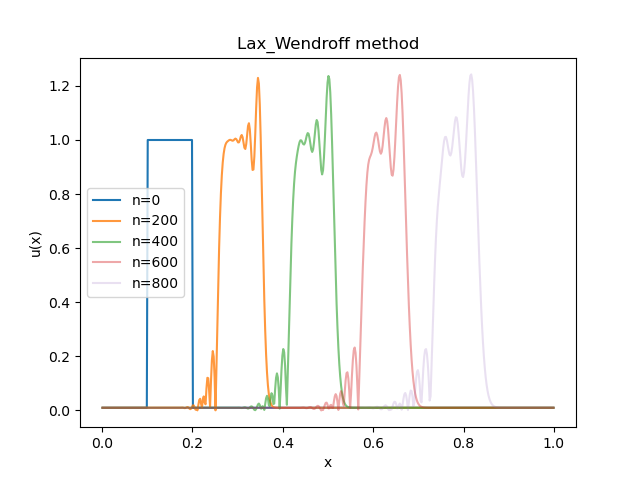
\includegraphics[width=0.7\textwidth]{LW_method} 
\caption{Lax-Wendroff method}  
\end{figure}

(2)Substituting the top hat function by Gaussian function, implement LW and LF method, the result:
\begin{figure}[H]
\centering  
\subfigure[Lax-Friedrich method]{
\includegraphics[width=0.45\textwidth]{G_LF_method}}
\subfigure[Lax-Wendroff method]{
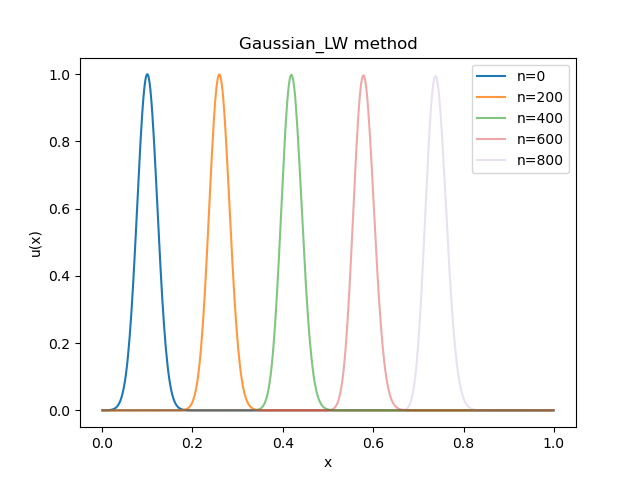
\includegraphics[width=0.45\textwidth]{G_LW_method}}
\caption{Gaussian function}
\end{figure}

(3)

\section{Exercise 3}
(1) Implemented the piecewise-linear method (PLM) for the advection test, the result figure:
\begin{figure}[H] 
\centering 
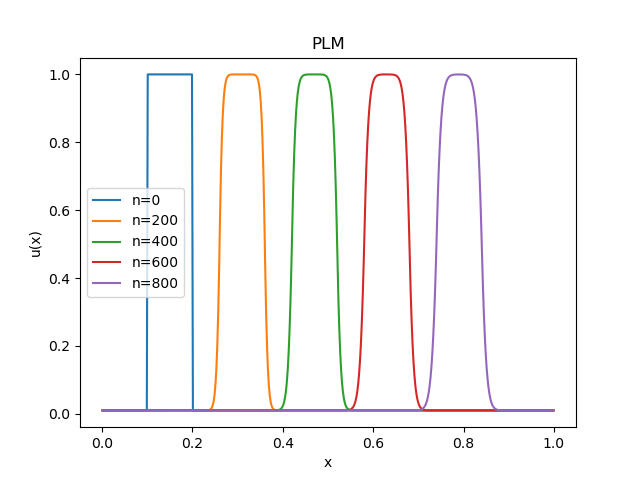
\includegraphics[width=0.7\textwidth]{PLM} 
\caption{Piecewise-linear method}  
\end{figure}

(2)Change 1-dimensional to 2-dimensional finite volume method, using PLM method to see how 2D advection go. Since the result animation can not be put here, I choose some screen shot as my result:
\begin{figure}[H]
\centering  
\subfigure[Square function going up-right (1)]{
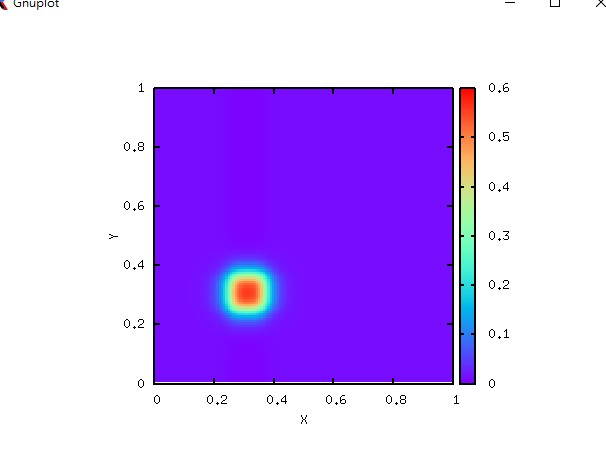
\includegraphics[width=0.45\textwidth]{EX3-1}}
\subfigure[Square function going up-right (2)]{
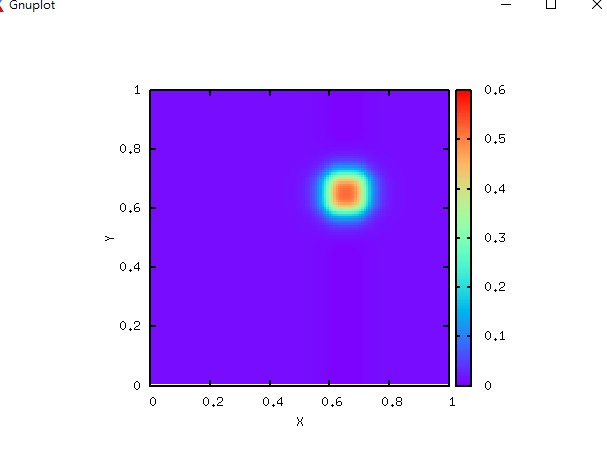
\includegraphics[width=0.45\textwidth]{EX3-2}}
\caption{2D advection simulation}
\end{figure}

\section{Exercise 4}




\section{Code link}
\href{https://github.com/kuo1235/Computational-Astrophysics-2022/tree/main/astr660/Homework/HW5/EX2/fvm}{\textcolor{blue}{\bf{Exercise2}}} 

\href{https://github.com/kuo1235/Computational-Astrophysics-2022/tree/main/astr660/Homework/HW5/EX3/fvm}{\textcolor{blue}{\bf{Exercise3-1}}}
\href{https://github.com/kuo1235/Computational-Astrophysics-2022/tree/main/astr660/Homework/HW5/EX3/fvm2d}{\textcolor{blue}{\bf{Exercise3-2}}}\\

\bibliography{Ref}
\end{document}







